% =====================================================================
%  MATH 55 -- Cheat Sheet for Topics 5-7 (Second Long Exam)
%  Every formula + how to match a function to its graph (MC items)
%  Build: latexmk -pdf -outdir=build cheat-sheet.tex
% =====================================================================
\documentclass[11pt,a4paper]{article}

\newcommand{\NotesNumber}{CS}
\newcommand{\NotesKind}{Cheat Sheet: Topics 5--7}
\newcommand{\NotesShortTitle}{Formulas and Graph Identification}
\newcommand{\NotesPdfTitle}{MATH 55 Cheat Sheet: Topics 5-7 Formulas and Graph Identification}
% =====================================================================
%  MATH 55 -- Shared preamble for the Second Long Exam reviewers
%  Reproduces the look of "Lecture Notes 01" (Lecture Notes & Reviewer
%  No. 5): Latin Modern, small-caps running heads, ruled chapter titles,
%  amsthm environments numbered within chapters, framed strategy boxes.
%
%  Each document defines, BEFORE \input-ing this file:
%     \NotesNumber      e.g. 6
%     \NotesKind        e.g. Lecture Notes \& Reviewer No.~6
%     \NotesShortTitle  e.g. Directional Derivatives and Gradient
%     \NotesPdfTitle    plain-text title for the PDF metadata
% =====================================================================

% ---------- Fonts and encoding --------------------------------------
\usepackage[T1]{fontenc}
\usepackage[utf8]{inputenc}
\usepackage{lmodern}
\usepackage{microtype}

% ---------- Page geometry -------------------------------------------
\usepackage[a4paper,top=1in,bottom=1in,left=1.05in,right=1.05in,
            headheight=15pt,footskip=30pt]{geometry}
\setlength{\parindent}{0pt}
\setlength{\parskip}{6pt plus 2pt minus 1pt}

% ---------- Mathematics ---------------------------------------------
\usepackage{amsmath,amssymb,amsthm,mathtools}
\usepackage{bm}

% ---------- Graphics, tables, lists ---------------------------------
\usepackage{graphicx}
\usepackage[dvipsnames]{xcolor}
\usepackage{tikz}
\usetikzlibrary{arrows.meta,calc,angles,quotes,positioning}
\usepackage{pgfplots}
\pgfplotsset{compat=1.17}
\usepackage{booktabs,array,tabularx,multirow}
\usepackage{caption}
\usepackage{subcaption}
\captionsetup{font=small,labelfont=bf,width=0.92\linewidth}
\usepackage{enumitem}
\setlist{itemsep=2pt,topsep=4pt}
\usepackage{float}
\usepackage[most]{tcolorbox}

% ---------- Headings --------------------------------------------------
\usepackage{titlesec}
% "Chapter N" over a ruled small-caps title, each on a new page
\titleformat{\section}[display]
  {\normalfont\centering}
  {\large\scshape Chapter \thesection}
  {8pt}
  {\titlerule\vspace{10pt}\LARGE\scshape}
  [\vspace{4pt}\titlerule]
\titlespacing*{\section}{0pt}{0pt}{22pt}
\newcommand{\sectionbreak}{\clearpage}
\titleformat{\subsection}{\normalfont\large\bfseries}{\thesubsection}{1em}{}
\titleformat{\subsubsection}{\normalfont\normalsize\bfseries}{\thesubsubsection}{1em}{}
\setcounter{tocdepth}{2}

% Appendices are titled "Appendix A" instead of "Chapter A"
\newcommand{\startappendix}{%
  \appendix
  \titleformat{\section}[display]
    {\normalfont\centering}
    {\large\scshape Appendix \thesection}
    {8pt}
    {\titlerule\vspace{10pt}\LARGE\scshape}
    [\vspace{4pt}\titlerule]%
}

% ---------- Running heads and feet ----------------------------------
\usepackage{fancyhdr}
\newcommand{\NotesAuthor}{Juevesano, D.}
\fancypagestyle{m55}{%
  \fancyhf{}%
  \fancyhead[L]{\small\textsc{\NotesKind}}%
  \fancyhead[R]{\small\textsc{Math 55 -- \NotesShortTitle}}%
  \fancyfoot[L]{\small\NotesAuthor\ 2026 ALL RIGHTS RESERVED. Not for redistribution.}%
  \fancyfoot[R]{\small\thepage}%
  \renewcommand{\headrulewidth}{0.4pt}%
  \renewcommand{\footrulewidth}{0.4pt}%
}
% chapter-opening pages use "plain": keep the same head/foot there too
\fancypagestyle{plain}{%
  \fancyhf{}%
  \fancyhead[L]{\small\textsc{\NotesKind}}%
  \fancyhead[R]{\small\textsc{Math 55 -- \NotesShortTitle}}%
  \fancyfoot[L]{\small\NotesAuthor\ 2026 ALL RIGHTS RESERVED. Not for redistribution.}%
  \fancyfoot[R]{\small\thepage}%
  \renewcommand{\headrulewidth}{0.4pt}%
  \renewcommand{\footrulewidth}{0.4pt}%
}
\pagestyle{m55}

% ---------- Theorem-like environments --------------------------------
\theoremstyle{definition}
\newtheorem{definition}{Definition}[section]
\newtheorem{example}[definition]{Example}
\newtheorem{problem}[definition]{Problem}
\newtheorem{exercise}[definition]{Exercise}
\theoremstyle{plain}
\newtheorem{theorem}[definition]{Theorem}
\newtheorem{proposition}[definition]{Proposition}
\newtheorem{corollary}[definition]{Corollary}
\newtheorem{lemma}[definition]{Lemma}
\theoremstyle{remark}
\newtheorem{remark}[definition]{Remark}
\newtheorem{warning}[definition]{Warning}

\newenvironment{solution}{\begin{proof}[Solution]}{\end{proof}}
% bold step labels inside solutions, e.g. \step{1}{Partial derivatives.}
\newcommand{\step}[2]{\par\smallskip\noindent\textbf{Step #1: #2}\ }
\newcommand{\stepx}[1]{\par\smallskip\noindent\textbf{#1}\ }
\newcommand{\checkok}{\ \checkmark}

% ---------- Boxes -----------------------------------------------------
% Framed "Strategy" box (as on p. 7 of Lecture Notes 01)
\newtcolorbox{strategy}[1]{%
  enhanced,breakable,colback=white,colframe=black!75,boxrule=0.6pt,
  sharp corners,left=10pt,right=10pt,top=8pt,bottom=8pt,
  before upper={\textbf{#1}\par\smallskip}}
% Highlighted key-result box
\newtcolorbox{keybox}[1]{%
  enhanced,breakable,colback=black!3,colframe=black!75,boxrule=0.6pt,
  sharp corners,left=10pt,right=10pt,top=8pt,bottom=8pt,
  before upper={\textbf{#1}\par\smallskip}}

% "Alternative method" box: a quicker route shown AFTER the full solution
\newtcolorbox{altmethod}{%
  enhanced,breakable,colback=white,colframe=black!45,boxrule=0.5pt,
  sharp corners,left=10pt,right=10pt,top=6pt,bottom=6pt,
  before upper={\textbf{Alternative method (optional).}\ }}
% Boxed concluding sentence of a solution
\newcommand{\finalans}[1]{\par\smallskip\noindent\textbf{Final answer.}\ #1}

% ---------- Notation --------------------------------------------------
\newcommand{\R}{\mathbb{R}}
\newcommand{\vb}[1]{\mathbf{#1}}
\newcommand{\vi}{\mathbf{i}}
\newcommand{\vj}{\mathbf{j}}
\newcommand{\vk}{\mathbf{k}}
\newcommand{\vu}{\mathbf{u}}
\newcommand{\vv}{\mathbf{v}}
\newcommand{\vr}{\mathbf{r}}
\newcommand{\vx}{\mathbf{x}}
\newcommand{\vF}{\mathbf{F}}
\newcommand{\vT}{\mathbf{T}}
\newcommand{\vN}{\mathbf{N}}
\newcommand{\vB}{\mathbf{B}}
\newcommand{\vzero}{\mathbf{0}}
\newcommand{\ip}[1]{\left\langle #1 \right\rangle}
\DeclarePairedDelimiter{\norm}{\lVert}{\rVert}
\DeclarePairedDelimiter{\abs}{\lvert}{\rvert}
\newcommand{\dd}{\mathrm{d}}
\newcommand{\Du}{D_{\mathbf{u}}}
\newcommand{\grad}{\nabla}
\newcommand{\pd}[2]{\frac{\partial #1}{\partial #2}}
\newcommand{\vecPQ}{\overrightarrow{PQ}}
\newcommand{\eval}[1]{\Big|_{#1}}

% ---------- Interactive links (underlined, like Lecture Notes 01) ----
\newcommand{\extlink}[2]{\href{#1}{\underline{#2}}}
\newcommand{\interactive}[2]{%
  \par\noindent\textit{Interactive:} \extlink{#1}{#2}\ }
\newcommand{\desmosTD}{https://www.desmos.com/3d}
\newcommand{\desmosTwoD}{https://www.desmos.com/calculator}

% ---------- Hyperref (load last) -------------------------------------
\usepackage[hidelinks]{hyperref}
\hypersetup{pdfauthor={Juevesano, D.},pdftitle={\NotesPdfTitle}}

% ---------- Title page -----------------------------------------------
% \makenotestitle{Title}{Subtitle}{Line under "No. N"}{About text}
\newcommand{\makenotestitle}[4]{%
  \begingroup
    \thispagestyle{plain}
    \centering
    \vspace*{1.6cm}
    {\large\scshape University of the Philippines Cebu\par
     Mathematics Program\par}
    \vspace{1.6cm}
    \rule{\linewidth}{0.5pt}\par\vspace{0.8cm}
    {\Huge\scshape #1\par}
    \vspace{0.5cm}
    {\large #2\par}
    \vspace{0.8cm}\rule{\linewidth}{0.5pt}\par
    \vspace{1.4cm}
    {\large\scshape \NotesKind\par}
    \vspace{0.4cm}
    {#3\par}
    \vfill
    \begin{minipage}{0.84\linewidth}
      \small\raggedright #4
    \end{minipage}
    \vfill
    {\NotesAuthor\quad 2026\par}
    \vspace{0.6cm}
  \clearpage
  \endgroup
}

% The table of contents is a starred \section, so it automatically gets
% the centred, ruled small-caps title used for chapters.

\graphicspath{{figures/}}

% compact tables for a cheat sheet
\newcolumntype{L}[1]{>{\raggedright\arraybackslash}p{#1}}
\newcolumntype{Y}{>{\raggedright\arraybackslash}X}
\newcommand{\fact}[2]{#1 & #2\\}

\begin{document}
\pagenumbering{roman}

\makenotestitle{Cheat Sheet}
  {Topics 5--7: Every Formula, and How to Match a Function to Its Graph}
  {MATH 55: Elementary Analysis III -- Second Long Examination}
  {\textbf{What this is.} A condensed reference for Slides~5 (Vector
   Functions), 6 (Directional Derivatives and the Gradient) and 7 (Vector
   Calculus, Parts I--III). Chapters~1--3 list every formula and the
   standard method for each problem type. Chapters~4--5 cover the
   multiple-choice items where you are given a function and have to pick its
   graph, or the other way round: a step-by-step checklist, a labelled gallery
   of the common curves and vector fields, and a reverse look-up table that
   goes from a feature of the picture to a feature of the formula. Chapter~6
   has practice items of that kind, with answers.\par\medskip
   \emph{Scope:} line integrals and the Fundamental Theorem for Line
   Integrals (Slides~7 Parts IV--VI) are not on this exam and are left out.
   For full explanations see Lecture Notes Nos.~5--7.}

\tableofcontents
\clearpage
\pagenumbering{arabic}

% =====================================================================
\section{Topic 5: Vector Functions}\label{ch:vf}
% =====================================================================

\subsection*{Core formulas}

\begin{center}
\renewcommand{\arraystretch}{1.45}
\begin{tabularx}{\linewidth}{L{0.28\linewidth}Y}
\toprule
\textbf{Concept} & \textbf{Formula / fact}\\
\midrule
\fact{Vector function}{$\vr(t)=\ip{f(t),g(t),h(t)}=f(t)\vi+g(t)\vj+h(t)\vk$. Its domain is the
  set of $t$ where \emph{all three} components are defined (intersect the domains).}
\fact{Space curve}{$C$ is the set of points $(f(t),g(t),h(t))$ traced by the tip of $\vr(t)$.
  Parametric equations: $x=f(t),\ y=g(t),\ z=h(t)$.}
\fact{Line through $P_0$, direction $\vv$}{$\vr(t)=\vr_0+t\vv$, \quad i.e.\ $x=x_0+at,\ y=y_0+bt,\ z=z_0+ct$.}
\fact{Segment from $\vr_0$ to $\vr_1$}{$\vr(t)=(1-t)\vr_0+t\,\vr_1,\quad 0\le t\le 1$ \ (start at $t=0$, end at $t=1$).}
\fact{Derivative}{$\vr'(t)=\lim_{h\to0}\dfrac{\vr(t+h)-\vr(t)}{h}=\ip{f'(t),g'(t),h'(t)}$ (differentiate each component).}
\fact{Tangent vector}{$\vr'(t_0)$ is tangent to $C$ at $\vr(t_0)$ (provided $\vr'(t_0)\ne\vzero$).}
\fact{Unit tangent}{$\vT(t)=\dfrac{\vr'(t)}{\norm{\vr'(t)}}$}
\fact{Tangent line at $t_0$}{$\vb{L}(s)=\vr(t_0)+s\,\vr'(t_0)$: \ point $=\vr(t_0)$, direction $=\vr'(t_0)$.}
\fact{Integral}{$\displaystyle\int_a^b\vr(t)\,\dd t=\ip{\int_a^b f,\int_a^b g,\int_a^b h}$ (a \emph{vector}).
  Indefinite: $\int\vr\,\dd t=\vb R(t)+\vb C$, with $\vb C$ a \emph{constant vector}.}
\fact{Initial value problem}{Integrate each component, then solve $\vb R(0)+\vb C=\vr(0)$ for $\vb C$.}
\fact{Smooth curve}{$\vr'$ continuous and $\vr'(t)\ne\vzero$ on the interval.}
\fact{Arc length}{$L=\displaystyle\int_a^b\norm{\vr'(t)}\,\dd t=\int_a^b\sqrt{f'^2+g'^2+h'^2}\,\dd t$ \quad
  (plane: $\int_a^b\sqrt{f'^2+g'^2}\,\dd t$).}
\fact{Arc length function}{$s(t)=\displaystyle\int_a^t\norm{\vr'(u)}\,\dd u,\qquad \dfrac{\dd s}{\dd t}=\norm{\vr'(t)}$.}
\fact{Curvature (definition)}{$\kappa=\norm*{\dfrac{\dd\vT}{\dd s}}=\dfrac{\norm{\vT'(t)}}{\norm{\vr'(t)}}$}
\fact{Curvature (use this)}{$\kappa(t)=\dfrac{\norm{\vr'(t)\times\vr''(t)}}{\norm{\vr'(t)}^3}$ \quad
  (for a plane curve put $0$ as the third component).}
\fact{Graph $y=f(x)$}{$\kappa(x)=\dfrac{\abs{f''(x)}}{\bigl(1+f'(x)^2\bigr)^{3/2}}$ \quad (from $\vr(x)=\ip{x,f(x),0}$).}
\fact{Ready-made curvatures}{Line: $\kappa=0$.\quad Circle of radius $a$: $\kappa=1/a$.\quad
  Helix $\ip{a\cos t,a\sin t,ct}$: $\kappa=\dfrac{a}{a^2+c^2}$.\quad $y=ax^2$ at $0$: $\kappa=2\abs a$.}
\bottomrule
\end{tabularx}
\end{center}

\subsection*{Differentiation rules}
For differentiable $\vu(t),\vv(t)$, scalar $c$ and real function $f(t)$:
\[
(\vu+\vv)'=\vu'+\vv',\quad (c\vu)'=c\vu',\quad (f\vu)'=f'\vu+f\vu',\quad
(\vu\cdot\vv)'=\vu'\cdot\vv+\vu\cdot\vv',
\]
\[
(\vu\times\vv)'=\vu'\times\vv+\vu\times\vv' \ (\text{keep the order}),\qquad
\bigl(\vu(f(t))\bigr)'=f'(t)\,\vu'(f(t)).
\]
If $\norm{\vr(t)}$ is constant then $\vr(t)\cdot\vr'(t)=0$; in particular $\vT\perp\vT'$.

\subsection*{Cross product (for the curvature formula)}
\[
\ip{a_1,a_2,a_3}\times\ip{b_1,b_2,b_3}
=\ip{a_2b_3-a_3b_2,\ \ a_3b_1-a_1b_3,\ \ a_1b_2-a_2b_1}.
\]

\subsection*{Methods for the standard problems}

\begin{strategy}{Curve of intersection of two surfaces (e.g.\ cylinder $\cap$ plane)}
\begin{enumerate}
\item Find the equation in only two variables (usually the cylinder, or eliminate a variable).
  It is a circle or an ellipse in that coordinate plane.
\item Parametrize it: $(x-h)^2+(y-k)^2=r^2\Rightarrow x=h+r\cos t,\ y=k+r\sin t$;
  \ $\frac{x^2}{a^2}+\frac{y^2}{b^2}=1\Rightarrow x=a\cos t,\ y=b\sin t$; \ $0\le t\le 2\pi$.
\item Solve the other surface for the remaining variable: e.g.\ plane $y+z=2\Rightarrow z=2-\sin t$.
\item Check the starting point and orientation the problem asks for. Viewed from above,
  $(\cos t,\sin t)$ runs counterclockwise from $(1,0)$; to start elsewhere shift $t$ or swap
  $\sin$ and $\cos$.
\end{enumerate}
\emph{Sphere $\cap$ plane through the origin} (Quiz~2): solve the plane for one variable, e.g.\
$3x-4z=0\Rightarrow z=\tfrac34x$, substitute into the sphere: $x^2+y^2+\tfrac9{16}x^2=25\Rightarrow
\frac{x^2}{16}+\frac{y^2}{25}=1$, an ellipse, so $x=4\cos t,\ y=5\sin t,\ z=3\cos t$.
\end{strategy}

\begin{strategy}{Move a distance $d$ along a curve (arc-length parametrization)}
Compute $s(t)=\int_{t_0}^t\norm{\vr'(u)}\,\dd u$, solve $s(t)=d$ for $t$, plug that $t$ into
$\vr$. \ Example: $\vr=\ip{3\sin t,4t,3\cos t}$, $\norm{\vr'}=\sqrt{9\cos^2t+16+9\sin^2t}=5$, so $s=5t$;
moving $5$ units from $(0,0,3)$ gives $t=1$, position $(3\sin1,\,4,\,3\cos1)$.
\end{strategy}

\begin{strategy}{Curvature at a point}
Find the $t$ for the point first. Compute $\vr'$, $\vr''$ at that $t$ (plug in \emph{before}
taking the cross product, to save algebra), then $\kappa=\norm{\vr'\times\vr''}/\norm{\vr'}^3$.
\end{strategy}

\subsection*{Common mistakes}
\begin{itemize}
\item Using $\vr'(t_0)$ as the point of the tangent line. The point is $\vr(t_0)$.
\item Forgetting that $\vT$ must be divided by $\norm{\vr'}$.
\item Forgetting the \emph{vector} constant $\vb C=\ip{C_1,C_2,C_3}$ when integrating.
\item In the arc length, integrating $\vr'$ instead of $\norm{\vr'}$, or using the wrong $t$-limits
  (convert the endpoints to $t$ values first).
\item Cubing the wrong thing in $\kappa$: the denominator is $\norm{\vr'}^{3}$, not $\norm{\vr''}^3$.
\end{itemize}

% =====================================================================
\section{Topic 6: Directional Derivatives and the Gradient}\label{ch:grad}
% =====================================================================

\subsection*{Core formulas}

\begin{center}
\renewcommand{\arraystretch}{1.45}
\begin{tabularx}{\linewidth}{L{0.28\linewidth}Y}
\toprule
\textbf{Concept} & \textbf{Formula / fact}\\
\midrule
\fact{Partial derivatives}{$f_x$ = rate of change in the $\vi$ direction, $f_y$ = rate of change in the $\vj$ direction.}
\fact{Directional derivative (definition)}{$\Du f(x_0,y_0)=\displaystyle\lim_{h\to0}\frac{f(x_0+ha,\,y_0+hb)-f(x_0,y_0)}{h}$,
  \ $\vu=\ip{a,b}$ a \textbf{unit} vector.}
\fact{Formula}{$\Du f(x,y)=f_x(x,y)\,a+f_y(x,y)\,b$ \quad ($f$ differentiable).}
\fact{Angle form}{If $\vu$ makes angle $\theta$ with the positive $x$-axis, $\vu=\ip{\cos\theta,\sin\theta}$ and
  $\Du f=f_x\cos\theta+f_y\sin\theta$.}
\fact{Gradient}{$\grad f=\ip{f_x,f_y}=f_x\vi+f_y\vj$; \quad in 3D $\grad f=\ip{f_x,f_y,f_z}$.}
\fact{Dot-product form}{$\Du f=\grad f\cdot\vu=\norm{\grad f}\cos\theta$ ($\theta$ = angle between $\grad f$ and $\vu$).}
\fact{Maximum rate}{$\max\Du f=\norm{\grad f}$, in the direction $\vu=\dfrac{\grad f}{\norm{\grad f}}$ (fastest increase).}
\fact{Minimum rate}{$\min\Du f=-\norm{\grad f}$, in the direction $-\grad f$ (fastest decrease).}
\fact{Zero rate}{$\Du f=0$ when $\vu\perp\grad f$: the direction \emph{along the level curve}.}
\fact{Possible values}{Every value of $\Du f$ lies in $\bigl[-\norm{\grad f},\ \norm{\grad f}\bigr]$.}
\fact{Direction from $P$ toward $Q$}{$\vu=\dfrac{\vecPQ}{\norm{\vecPQ}}$ (always normalise!).}
\fact{Geometry}{$\grad f(P)$ is \emph{perpendicular} to the level curve $f=f(P)$ through $P$ and points toward
  \emph{larger} values of $f$.}
\fact{Tangent plane to $F(x,y,z)=k$}{$\grad F(P)\cdot\ip{x-x_0,y-y_0,z-z_0}=0$; normal line $\vr(t)=P+t\,\grad F(P)$.}
\fact{Chain rule (along a curve)}{$\dfrac{\dd}{\dd t}f(\vr(t))=\grad f(\vr(t))\cdot\vr'(t)$.}
\bottomrule
\end{tabularx}
\end{center}

\subsection*{Methods for the standard problems}

\begin{strategy}{Directional derivative at $P$ toward $Q$ (Quiz~2, Problem~2)}
\begin{enumerate}
\item $\grad f=\ip{f_x,f_y}$, then evaluate at $P$.
\item $\vv=\vecPQ=Q-P$, \ $\vu=\vv/\norm{\vv}$.
\item $\Du f(P)=\grad f(P)\cdot\vu$.
\item Fastest increase: unit vector $\grad f(P)/\norm{\grad f(P)}$. Maximum rate: $\norm{\grad f(P)}$.
\end{enumerate}
\end{strategy}

\begin{strategy}{Find the directions in which $\Du f(P)=c$ (Quiz~2, Problem~5)}
Let $\vu=\ip{a,b}$ and $\grad f(P)=\ip{p,q}$. Solve the system
\[ pa+qb=c,\qquad a^2+b^2=1. \]
Substitute the linear equation into the circle: 0, 1 or 2 unit vectors. Solutions exist only if
$\abs c\le\norm{\grad f(P)}$; if $\abs c=\norm{\grad f(P)}$ there is exactly one (namely
$\pm\grad f/\norm{\grad f}$). \ Shortcut: $\cos\theta=c/\norm{\grad f}$ gives the angle between
$\vu$ and $\grad f$; rotate $\grad f$ by $\pm\theta$.
\end{strategy}

\begin{strategy}{Points where the fastest increase is in a given direction $\vv$ (Quiz~2, Problem~6)}
Require $\grad f(x,y)=\lambda\vv$ with $\lambda>0$ (same direction, not opposite). E.g.\
$f=x^2+y^2-2x-4y$, $\vv=\vi+\vj$: $\ip{2x-2,2y-4}=\ip{\lambda,\lambda}$ gives
$2x-2=2y-4>0$, i.e.\ the points on the line $y=x+1$ with $x>1$.
\end{strategy}

\subsection*{Common mistakes}
\begin{itemize}
\item Using a direction vector that is not a unit vector. ($\ip{3,-4}$ must become $\ip{\frac35,-\frac45}$.)
\item Writing the \emph{maximum rate} as a vector. It is the number $\norm{\grad f}$; the
  \emph{direction} is the vector.
\item Evaluating the gradient at $Q$ instead of $P$.
\item Accepting $\lambda<0$ in ``direction of fastest increase is $\vv$'': that is fastest \emph{decrease}.
\end{itemize}

% =====================================================================
\section{Topic 7: Vector Fields and Conservative Fields}\label{ch:fields}
% =====================================================================

\subsection*{Core formulas}

\begin{center}
\renewcommand{\arraystretch}{1.45}
\begin{tabularx}{\linewidth}{L{0.28\linewidth}Y}
\toprule
\textbf{Concept} & \textbf{Formula / fact}\\
\midrule
\fact{Vector field on $\R^2$}{$\vF(x,y)=\ip{M(x,y),N(x,y)}=M\vi+N\vj$: assigns a vector to each point.}
\fact{Vector field on $\R^3$}{$\vF(x,y,z)=\ip{M,N,P}=M\vi+N\vj+P\vk$.}
\fact{Position notation}{$\vx=\ip{x,y}$ (or $\ip{x,y,z}$), so $\vF(\vx)$ means $\vF(x,y)$; \ $\norm{\vx}=r$.}
\fact{Sketching}{Draw the arrow $\vF(x,y)$ \emph{starting at the point} $(x,y)$, not at the origin.}
\fact{Gradient field}{$\grad f=\ip{f_x,f_y}$ or $\ip{f_x,f_y,f_z}$ is a vector field.}
\fact{Conservative}{$\vF$ is conservative if $\vF=\grad f$ for some $f$; $f$ is a \emph{potential function}
  (unique up to $+C$).}
\fact{Test in the plane}{$\vF=\ip{M,N}$ conservative $\iff \dfrac{\partial M}{\partial y}=\dfrac{\partial N}{\partial x}$
  (on an open disk / region without holes).}
\fact{Test in space}{$\vF=\ip{M,N,P}$ conservative $\iff M_y=N_x,\ \ M_z=P_x,\ \ N_z=P_y$ (all three!).}
\fact{Why the test works}{If $\vF=\grad f$ then $M_y=f_{xy}=f_{yx}=N_x$ (Clairaut).}
\fact{Rotation field}{$\ip{-y,x}$: $M_y=-1\ne1=N_x$, so it is \emph{not} conservative.}
\fact{Useful potentials}{$\grad\bigl(\tfrac12(x^2+y^2+z^2)\bigr)=\ip{x,y,z}$;\quad
  $\grad\tfrac1r=-\dfrac{\vx}{r^3}$;\quad $\grad\tfrac12\ln(x^2+y^2+z^2)=\dfrac{\vx}{r^2}$;\quad
  $\grad(xy)=\ip{y,x}$;\quad $\grad(x^3+\tfrac12y^2)=\ip{3x^2,y}$.}
\bottomrule
\end{tabularx}
\end{center}

\begin{strategy}{Finding a potential function (three-step method)}
\begin{enumerate}
\item Check the test ($M_y=N_x$, and in 3D the other two). If it fails, stop: not conservative.
\item $f=\int M\,\dd x+g(y,z)$ (a \emph{function} of the other variables, not a constant).
\item Differentiate: set $f_y=N$ to find $g$ up to $h(z)$; then $f_z=P$ to find $h$.
  If $g'(y)$ still contains $x$, there is a mistake.
\item Check: $\grad f=\vF$.
\end{enumerate}
Example: $\vF=\ip{2xy,\ x^2+3y^2}$. $M_y=2x=N_x$ \checkok. $f=x^2y+g(y)$, $f_y=x^2+g'(y)=x^2+3y^2\Rightarrow g=y^3$.
So $f=x^2y+y^3+C$.
\end{strategy}

\subsection*{Common mistakes}
\begin{itemize}
\item Comparing $M_x$ with $N_y$. The test pairs $M_y$ with $N_x$ (cross partials).
\item In 3D, checking only one pair.
\item Writing $+C$ instead of $+g(y)$ after the first integration.
\item The test needs a region without holes: $\vF=\dfrac{\ip{-y,x}}{x^2+y^2}$ passes $M_y=N_x$ but is not
  conservative on the plane minus the origin.
\end{itemize}

% =====================================================================
\section{Matching a Vector Function to Its Curve}\label{ch:curves}
% =====================================================================

Multiple-choice items usually show four 3D curves and one formula, or one curve and four
formulas. You almost never need to plot. Run through the checklist below until only one
option is left; usually two or three steps are enough.

\begin{keybox}{The 7-step checklist for space curves $\vr(t)=\ip{x(t),y(t),z(t)}$}
\begin{enumerate}
\item \textbf{Are all components linear in $t$?} Then the curve is a \emph{straight line}
  (or a segment if $t$ is restricted).
\item \textbf{Find the ``circle pair''.} If two components are $a\cos t$ and $a\sin t$, then
  $x^2+y^2=a^2$: the curve lies on a \emph{cylinder} around the third axis, and viewed down
  that axis it is a circle. With $a\cos t,\ b\sin t$ it is an ellipse (elliptical cylinder).
\item \textbf{What does the third component do?}
  \begin{itemize}
  \item $=t$ (or $ct$): climbs steadily, so a \emph{helix} around that axis.
  \item periodic with the same period ($\sin t$, $\cos t$, $2-\sin t$): a \emph{closed loop}
    lying in a tilted plane, i.e.\ an \emph{ellipse}.
  \item $\cos 2t$, $\sin^2t$, \dots\ (twice as fast): \emph{2 ups and 2 downs} per turn (a
    ``pringle'' or saddle-shaped loop). $\cos nt$: $n$ ups per turn.
  \item $e^{ct}$: climbs faster and faster, so the coils get \emph{farther apart}.
  \item $\frac1{1+t^2}$: one bump near $t=0$, then flattens out (the curve circles at a
    nearly constant height).
  \end{itemize}
\item \textbf{Is the radius growing?} If the circle pair is $t\cos t,\ t\sin t$ then
  $x^2+y^2=t^2$; together with $z=t$ that is $x^2+y^2=z^2$: a \emph{cone} (conical helix).
  The variable that appears alone ($z=t$ here) is the axis of the cone.
\item \textbf{Look for algebraic relations.} $y=x^2$, $z=x^3$ (twisted cubic $\ip{t,t^2,t^3}$);
  $x+y=1$ (the curve lies in a plane); $x^2+y^2+z^2=$ const (the curve lies on a sphere).
\item \textbf{Check signs and bounds.} $t^2\ge0$ and $e^t>0$, so that coordinate is never
  negative. $\abs{\sin},\abs{\cos}\le1$ keep the curve inside a box. $\cos^2t,\sin^2t\in[0,1]$.
\item \textbf{Plug in $t=0$ (and maybe $t=\frac\pi2$).} This gives the starting point and
  usually eliminates the remaining look-alikes. For orientation, compare two values of $t$.
\end{enumerate}
\end{keybox}

\subsection*{Orientation and start point at a glance}

\begin{center}
\renewcommand{\arraystretch}{1.35}
\begin{tabular}{lll}
\toprule
\textbf{Pair $(x,y)$} & \textbf{Start ($t=0$)} & \textbf{Direction (viewed from above, $+z$)}\\
\midrule
$(\cos t,\ \sin t)$ & $(1,0)$ & counterclockwise\\
$(\sin t,\ \cos t)$ & $(0,1)$ & clockwise\\
$(\cos t,\ -\sin t)$ & $(1,0)$ & clockwise\\
$(-\cos t,\ \sin t)$ & $(-1,0)$ & clockwise\\
$(\cos(-t),\ \sin(-t))$ & $(1,0)$ & clockwise (reversing $t$ reverses direction)\\
\bottomrule
\end{tabular}
\end{center}

Rule: \emph{swapping} $\sin$ and $\cos$, or putting a minus sign on exactly one of them,
\emph{reverses} the direction.

\subsection*{Which axis is the curve wrapped around?}

The axis is the coordinate that is \emph{not} in the $\cos/\sin$ pair:
\[
\ip{\cos t,\sin t,t}\ \to\ z\text{-axis},\qquad
\ip{t,\cos t,\sin t}\ \to\ x\text{-axis},\qquad
\ip{\cos t,t,\sin t}\ \to\ y\text{-axis}.
\]

\subsection*{Projections onto the coordinate planes}
To see the curve ``from above'' drop $z$; ``from the front'' drop $y$; ``from the side'' drop $x$.
For the helix $\ip{\cos t,\sin t,t}$: from above a circle, from the side a sine wave
($y=\sin z$), from the front a cosine wave ($x=\cos z$). MC items sometimes show one of these
2D views instead of the 3D curve.

\subsection*{Gallery: formula $\to$ picture}

In each panel the red dot is the point at $t=0$ (or the left end of the interval) and the
thick red piece shows the direction of increasing $t$.

\begin{figure}[H]
  \centering
  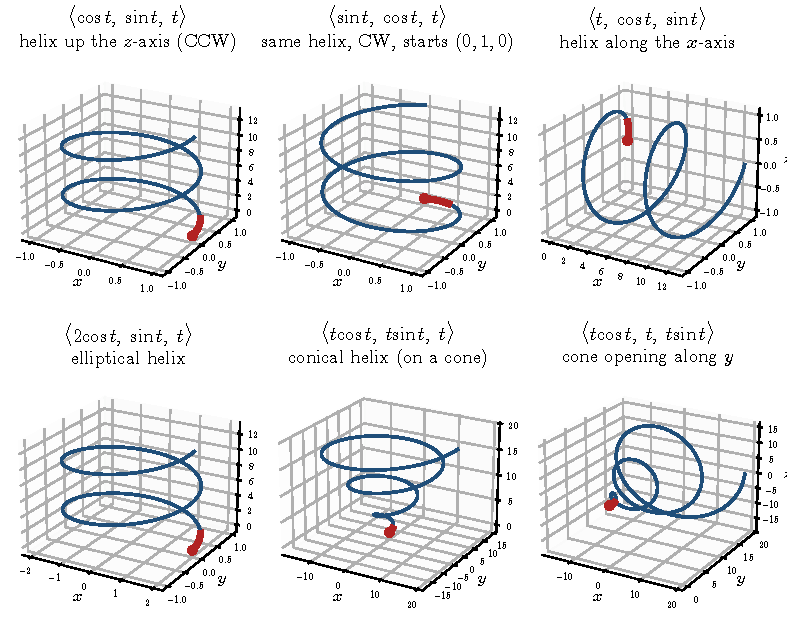
\includegraphics[width=\linewidth]{curves_gallery_1}
  \caption{Helices: circle pair + steadily increasing third component.
  The variable that appears alone is the axis.}
  \label{fig:curves1}
\end{figure}

\begin{figure}[H]
  \centering
  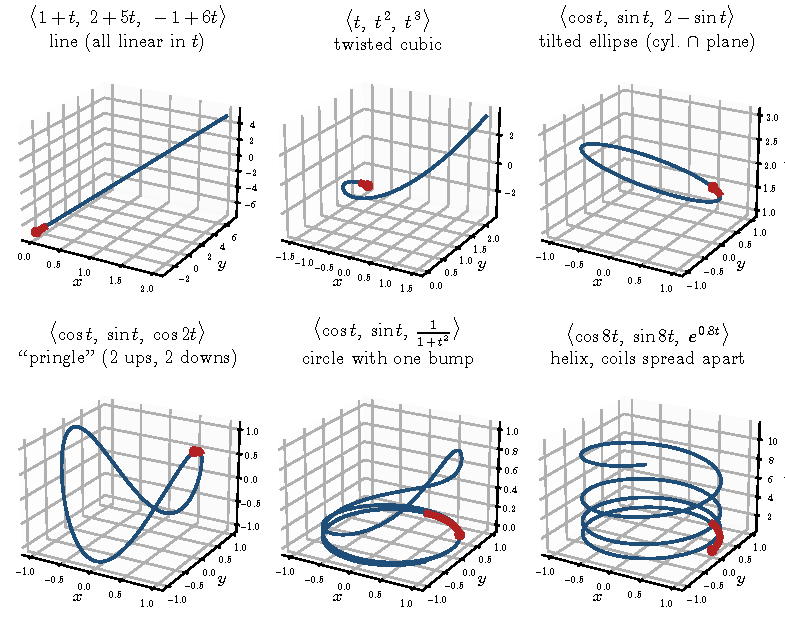
\includegraphics[width=\linewidth]{curves_gallery_2}
  \caption{Lines, the twisted cubic, closed loops on the cylinder $x^2+y^2=1$, and
  helices whose height is not linear in $t$.}
  \label{fig:curves2}
\end{figure}

\begin{figure}[H]
  \centering
  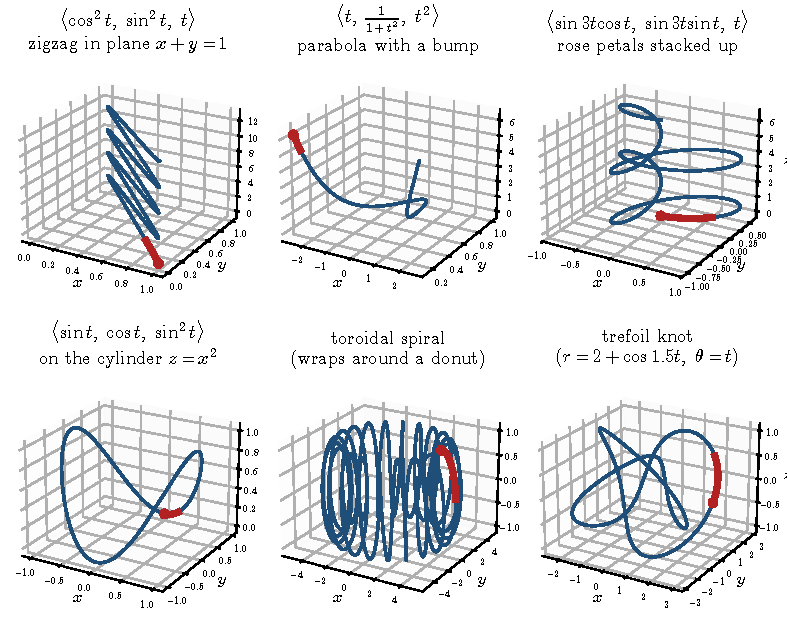
\includegraphics[width=\linewidth]{curves_gallery_3}
  \caption{More shapes that appear in matching items, including the two computer-drawn
  curves from the slides (toroidal spiral and trefoil knot).}
  \label{fig:curves3}
\end{figure}

\subsection*{Reverse look-up: picture $\to$ formula}

\begin{center}
\renewcommand{\arraystretch}{1.4}
\begin{tabularx}{\linewidth}{L{0.42\linewidth}Y}
\toprule
\textbf{If the picture shows\dots} & \textbf{look for a formula with\dots}\\
\midrule
a straight line & every component linear: $\ip{x_0+at,\ y_0+bt,\ z_0+ct}$\\
a spring with equal spacing & a $\cos t/\sin t$ pair and the third component $=ct$\\
a spring whose coils spread apart & third component growing faster than linear ($e^{t}$, $t^2$)\\
a spring that widens (cone) & pair $t\cos t,\ t\sin t$ (radius $=t$)\\
a flat closed loop, tilted & pair $\cos t,\sin t$ and third component $=a+b\cos t+c\sin t$\\
a closed loop going up--down--up--down & third component $\cos2t$, $\sin2t$, $\sin^2t$, $\cos^2t$\\
a circle with one bump that settles & third component $\frac1{1+t^2}$ (or $e^{-t^2}$)\\
an S-shaped curve through the origin & polynomial components like $\ip{t,t^2,t^3}$\\
a curve that stays on one side ($z\ge0$) & a component such as $t^2$, $e^t$, $\sin^2t$\\
a curve that wraps a donut & $\bigl((R+\sin nt)\cos t,\ (R+\sin nt)\sin t,\ \cos nt\bigr)$\\
\bottomrule
\end{tabularx}
\end{center}

\subsection*{2D curves from Topic 5 (parametric plane curves)}

\begin{center}
\renewcommand{\arraystretch}{1.35}
\begin{tabularx}{\linewidth}{L{0.42\linewidth}Y}
\toprule
\textbf{Parametrization} & \textbf{Curve}\\
\midrule
$\ip{h+r\cos t,\ k+r\sin t}$ & circle, centre $(h,k)$, radius $r$, CCW\\
$\ip{a\cos t,\ b\sin t}$ & ellipse $\frac{x^2}{a^2}+\frac{y^2}{b^2}=1$\\
$\ip{t,\ f(t)}$ & the graph $y=f(x)$\\
$\ip{t^2-2t,\ t+1}$ (slides) & eliminate $t$: $t=y-1$, $x=(y-1)^2-2(y-1)$, a sideways parabola\\
$\ip{a\cosh t,\ b\sinh t}$ & right branch of a hyperbola ($\cosh^2-\sinh^2=1$)\\
\bottomrule
\end{tabularx}
\end{center}
To identify a plane curve, \emph{eliminate $t$}: use $\cos^2t+\sin^2t=1$ for trig pairs, or
solve one equation for $t$ and substitute into the other.

% =====================================================================
\section{Matching a Vector Field (or Gradient) to Its Plot}\label{ch:idfields}
% =====================================================================

\begin{keybox}{The 6-step checklist for $\vF(x,y)=\ip{M,N}$}
\begin{enumerate}
\item \textbf{Plug in four test points}: $(1,0)$, $(0,1)$, $(-1,0)$, $(0,-1)$. Draw those four
  arrows in your head and compare. This alone decides most items.
\item \textbf{Constant?} If $M$ and $N$ are numbers, every arrow is the same (parallel, equal
  length).
\item \textbf{What does it depend on?} If $\vF$ depends only on $y$, every \emph{row}
  (horizontal line) of arrows is identical; depending only on $x$, every \emph{column} is.
\item \textbf{Radial or rotating?} $\vF$ parallel to $\ip{x,y}$ means radial (out if the
  multiple is positive, in if negative). $\vF\cdot\ip{x,y}=0$ means tangent to circles,
  i.e.\ rotating: $\ip{-y,x}$ is counterclockwise, $\ip{y,-x}$ clockwise.
\item \textbf{How does the length change?} $\norm{\ip{x,y}}=r$ grows outward;
  $\vx/\norm{\vx}$ has length 1 everywhere; $\vx/\norm{\vx}^3$ has length $1/r^2$ and is huge
  near the origin and tiny far away.
\item \textbf{Where is $\vF=\vzero$?} Solve $M=0,\ N=0$. A field like $\ip{x,y}$ vanishes only
  at the origin; $\ip{y,0}$ vanishes on the whole $x$-axis.
\end{enumerate}
Sign-of-components shortcut: in each quadrant, $M>0$ means the arrow points right, $N>0$ means
it points up.
\end{keybox}

\begin{figure}[H]
  \centering
  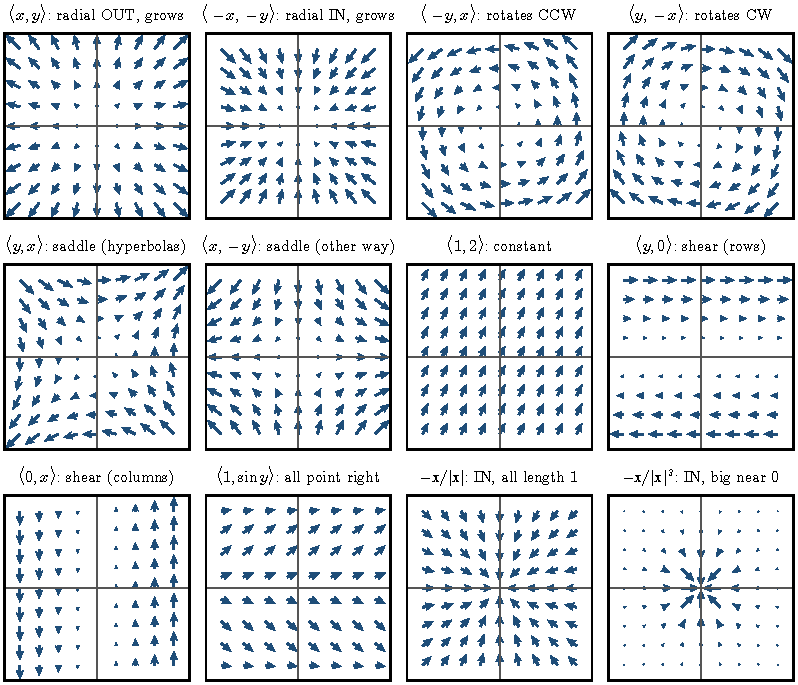
\includegraphics[width=\linewidth]{fields_gallery}
  \caption{The twelve fields that cover almost every matching item. (The last panel is
  capped near the origin so that the arrows stay visible.)}
  \label{fig:fieldsgallery}
\end{figure}

\subsection*{Quick reference: formula $\to$ look}

\begin{center}
\renewcommand{\arraystretch}{1.35}
\begin{tabularx}{\linewidth}{L{0.3\linewidth}Y}
\toprule
\textbf{Field} & \textbf{What the plot looks like}\\
\midrule
$\ip{x,y}$, $c\ip{x,y}$ ($c>0$) & arrows point away from the origin, longer farther out\\
$\ip{-x,-y}$ & arrows point toward the origin, longer farther out\\
$-\vx/\norm{\vx}$ & toward the origin, all the same length\\
$-\vx/\norm{\vx}^3$ (gravity) & toward the origin, very long near it, very short far away\\
$\ip{-y,x}$ & counterclockwise circles, longer farther out\\
$\ip{y,-x}$ & clockwise circles\\
$\ip{-y,x}/(x^2+y^2)$ & counterclockwise circles, \emph{shorter} farther out (vortex)\\
$\ip{y,x}$, $\ip{x,-y}$ & saddle (hyperbolic) pattern: in along one diagonal or axis, out along the other\\
$\ip{a,b}$ & all arrows identical\\
$\ip{y,0}$ & horizontal arrows: right above the $x$-axis, left below, zero on it\\
$\ip{0,x}$ & vertical arrows: up to the right of the $y$-axis, down to the left\\
$\ip{1,\sin y}$ & all point right, tilting up or down in horizontal bands\\
\bottomrule
\end{tabularx}
\end{center}

\subsection*{Vector fields in 3D (slides, Exercise 3)}

Use the same idea: look at what happens on the $z$-axis and as you move away from it.

\begin{figure}[H]
  \centering
  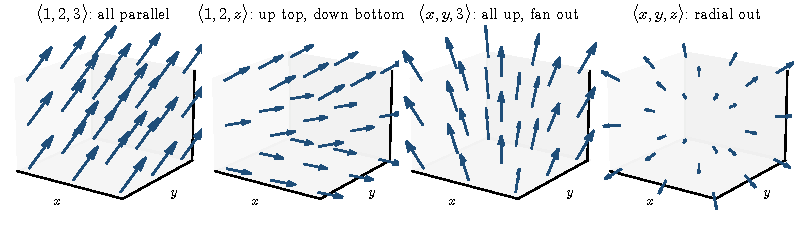
\includegraphics[width=\linewidth]{fields3d_gallery}
  \caption{$\ip{1,2,3}$: constant. $\ip{1,2,z}$: the $z$-component flips sign at $z=0$.
  $\ip{x,y,3}$: always upward, fanning away from the $z$-axis (the slide's answer, C).
  $\ip{x,y,z}$: radial from the origin, so the arrows below $z=0$ point down.}
  \label{fig:fields3d}
\end{figure}

\subsection*{Gradient fields and contour maps}

When the picture is a \emph{contour map} (level curves of $f$), or you must match $f$ to the
plot of $\grad f$:

\begin{keybox}{Rules for gradients on a contour map}
\begin{enumerate}
\item $\grad f$ is \emph{perpendicular} to the level curves.
\item $\grad f$ points toward \emph{higher} values of $f$ (uphill).
\item $\norm{\grad f}$ is \emph{larger} where the level curves are \emph{closer together}.
\item $\Du f>0$ if $\vu$ points uphill (to higher contours), $<0$ if downhill, $=0$ along a contour.
\item Peaks/valleys (closed circles around a point): $\grad f$ points in toward a maximum and out
  from a minimum. At the max/min itself, $\grad f=\vzero$.
\item To match $f$ with a plot of $\grad f$: compute $\grad f$, then use the 6-step checklist.
  A gradient field is conservative, so it \emph{never circulates}: a plot with arrows going
  around in closed loops is \emph{not} a gradient field.
\end{enumerate}
\end{keybox}

\begin{figure}[H]
  \centering
  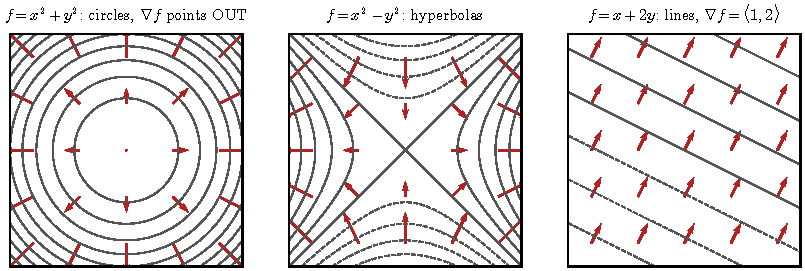
\includegraphics[width=\linewidth]{contours_gradient}
  \caption{Level curves (grey) with gradient vectors (red). The gradient is always
  perpendicular to the level curves and points to larger values. Dashed contours are
  negative levels.}
  \label{fig:contours}
\end{figure}

\subsection*{Level curves to recognise}
\begin{center}
\renewcommand{\arraystretch}{1.35}
\begin{tabularx}{\linewidth}{L{0.36\linewidth}Y}
\toprule
$f(x,y)$ & level curves $f=k$\\
\midrule
$ax+by$ & parallel lines, perpendicular to $\ip{a,b}$\\
$x^2+y^2$ & circles centred at the origin\\
$x^2+2y^2$, $ax^2+by^2$ ($a,b>0$) & ellipses\\
$x^2-y^2$, $xy$ & hyperbolas (plus two crossing lines for $k=0$)\\
$y-x^2$ & parabolas $y=x^2+k$\\
$\sqrt{x^2+y^2}$ vs.\ $x^2+y^2$ & both give circles. For $\sqrt{x^2+y^2}$ (a cone) equally spaced levels give \emph{evenly spaced}
  circles; for $x^2+y^2$ (a paraboloid) the circles get \emph{closer together} farther out\\
\bottomrule
\end{tabularx}
\end{center}

% =====================================================================
\section{Practice: Graph-Identification Items}\label{ch:drills}
% =====================================================================

Try each item using the checklists from Chapters~\ref{ch:curves}--\ref{ch:idfields} before
looking at the answers at the end of the chapter.

\subsection*{Picture items}

\textbf{1.} Which curve is $\vr(t)=\ip{t\cos t,\ t\sin t,\ t}$, $t\ge0$?
\begin{center}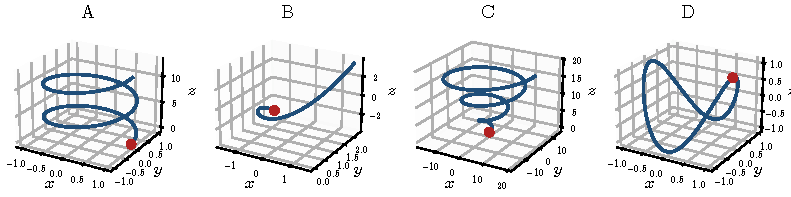
\includegraphics[width=0.95\linewidth]{drill_curves}\end{center}

\textbf{2.} Which curve is $\vr(t)=\ip{\cos t,\ \sin t,\ 2-\sin t}$, $0\le t\le2\pi$?
(The red dot is the point at $t=0$.)
\begin{center}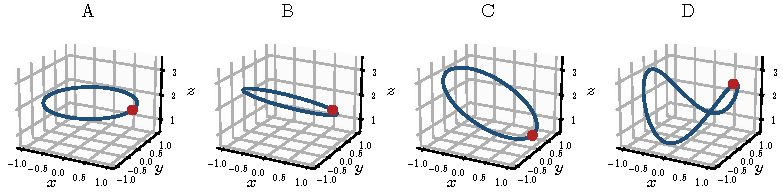
\includegraphics[width=0.95\linewidth]{drill_curves2}\end{center}

\textbf{3.} Match each field with its plot I--IV:\quad
(a) $\ip{x,-y}$\quad (b) $\ip{1,x}$\quad (c) $\ip{y,-x}$\quad (d) $\ip{-x,-y}$.
\begin{center}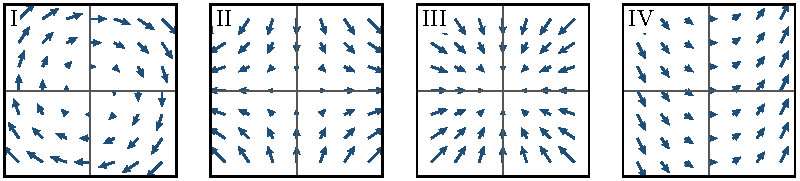
\includegraphics[width=0.95\linewidth]{drill_fields}\end{center}

\textbf{4.} Which plot is the gradient field of $f(x,y)=x^2y$? (All arrows are drawn with the
same length; only the directions matter.)
\begin{center}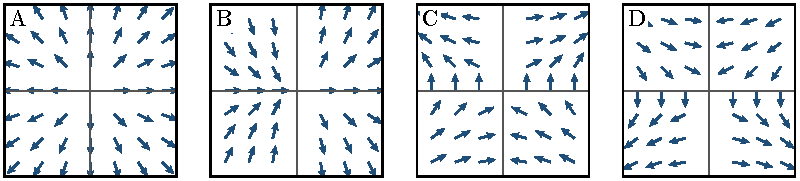
\includegraphics[width=0.95\linewidth]{drill_gradient}\end{center}

\textbf{5.} The contour map of $f$ is shown below (levels labelled).
\begin{center}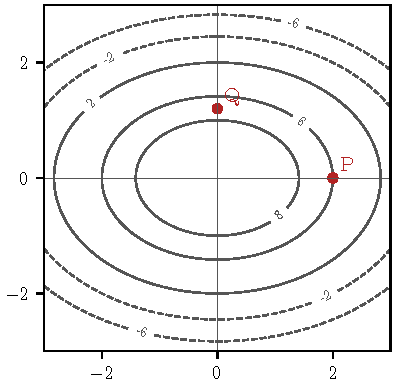
\includegraphics[width=0.36\linewidth]{drill_contour}\end{center}
(a) Is $D_{\vi}f(P)$ positive, negative or zero?\quad
(b) In which direction does $\grad f(Q)$ point?\quad
(c) Give a unit vector $\vu$ with $\Du f(P)=0$.\quad
(d) Does $f$ have a maximum or a minimum at the origin?

\subsection*{Formula-only items}

\begin{enumerate}[label=\textbf{\arabic*.},start=6]
\item Which curve lies on the cone $z^2=x^2+y^2$?\\
  A.\ $\ip{\cos t,\sin t,t}$\quad B.\ $\ip{t\cos t,t\sin t,t}$\quad C.\ $\ip{t,t^2,t^3}$\quad D.\ $\ip{\cos t,t,\sin t}$
\item Viewed from above, $\vr(t)=\ip{\sin t,\cos t,t}$ starts at \underline{\hspace{2cm}} and turns
  \underline{\hspace{2.5cm}}.
\item The helix $\ip{t,\ 3\cos t,\ 3\sin t}$ winds around which axis?
\item The curve $\ip{\cos^2t,\ \sin^2t,\ t}$ lies in which plane?
\item Which curve has curvature $0$ everywhere?\\
  A.\ $\ip{2t,1-t,3+4t}$\quad B.\ $\ip{t,t^2,0}$\quad C.\ $\ip{\cos t,\sin t,0}$\quad D.\ $\ip{t,t^3,t}$
\item Which field is conservative?\\
  A.\ $\ip{-y,x}$\quad B.\ $\ip{y,x}$\quad C.\ $\ip{y,-x}$\quad D.\ $\ip{x^2,xy}$
\item A plot shows arrows tangent to circles about the origin, turning counterclockwise and
  getting \emph{shorter} away from the origin. Which field?\\
  A.\ $\ip{-y,x}$\quad B.\ $\ip{y,-x}$\quad C.\ $\dfrac{\ip{-y,x}}{x^2+y^2}$\quad D.\ $\dfrac{\ip{x,y}}{x^2+y^2}$
\item Domain of $\vr(t)=\ip{\sqrt{4-t^2},\ \ln t,\ \dfrac1{t-1}}$?
\item A plot shows every arrow pointing straight up or straight down, up for $x>0$ and down for
  $x<0$. Which field?\quad A.\ $\ip{x,0}$\quad B.\ $\ip{0,x}$\quad C.\ $\ip{0,y}$\quad D.\ $\ip{y,0}$
\end{enumerate}

\subsection*{Answers}

\begin{enumerate}[label=\textbf{\arabic*.}]
\item \textbf{C.} $x^2+y^2=t^2=z^2$: a cone, so the spiral widens as it climbs. A has constant
  radius (ordinary helix), B is the twisted cubic, D is a closed loop.
\item \textbf{B.} At $t=0$ the point is $(1,0,2)$, which rules out C (starts at $z=1$) and D
  (starts at $z=3$). $z$ is not constant, which rules out A. Also $z=2-y$: highest at $y=-1$, so the
  loop is tilted along the $y$-direction, as in B.
\item (a) \textbf{II}, (b) \textbf{IV}, (c) \textbf{I}, (d) \textbf{III}.
  Test points: $\ip{y,-x}$ at $(0,1)$ is $\ip{1,0}$ (right, on top), so clockwise: I.
  $\ip{-x,-y}$ points inward: III. $\ip{x,-y}$ at $(1,0)$ points right but at $(0,1)$ points
  down: saddle, II. $\ip{1,x}$ always has $M=1$ (rightward) and tilts up for $x>0$: IV.
\item \textbf{C.} $\grad f=\ip{2xy,\ x^2}$. Its $y$-component $x^2\ge0$, so no arrow points
  down (rules out D), and on the $x$-axis ($y=0$) the arrows point straight up. A is
  $\grad(x^2+y^2)$ (radial); B has the components swapped ($\ip{x^2,2xy}$ always points right).
\item (a) \textbf{Negative}: moving right from $P$ goes to lower contours (6, then 2).
  (b) Straight \textbf{down}, toward the origin: perpendicular to the level curve and toward
  larger values (here $f=10-x^2-2y^2$, so $\grad f(Q)=\ip{0,-4.8}$). (c) $\vu=\pm\vj$ (tangent
  to the level curve at $P$). (d) A \textbf{maximum}: the levels increase toward the centre.
\item \textbf{B.}
\item $(0,1,0)$; \textbf{clockwise}.
\item The \textbf{$x$-axis} ($x=t$ is the variable that appears alone).
\item $x+y=\cos^2t+\sin^2t=1$: the plane \boldmath$x+y=1$\unboldmath.
\item \textbf{A} (all components linear, so it is a line).
\item \textbf{B.} $M_y=1=N_x$; potential $f=xy$. (A and C rotate; D: $M_y=0\ne y=N_x$.)
\item \textbf{C.} The length is $r/r^2=1/r$, so it shrinks; A grows, B is clockwise, D is radial.
\item Need $4-t^2\ge0$, $t>0$, $t\ne1$: \ \boldmath$(0,1)\cup(1,2]$\unboldmath.
\item \textbf{B.}
\end{enumerate}


\end{document}
